\documentclass[border=4pt]{standalone}
\usepackage{amsmath,amssymb,bm,mathtools}
\usepackage{tikz}
\usetikzlibrary{positioning,calc,decorations.pathreplacing,arrows.meta,fit,backgrounds}
\usepackage{xcolor}
\definecolor{blue}{HTML}{1F618D}\definecolor{red}{HTML}{B03A2E}\definecolor{gray}{HTML}{7F7F7F}
\begin{document}
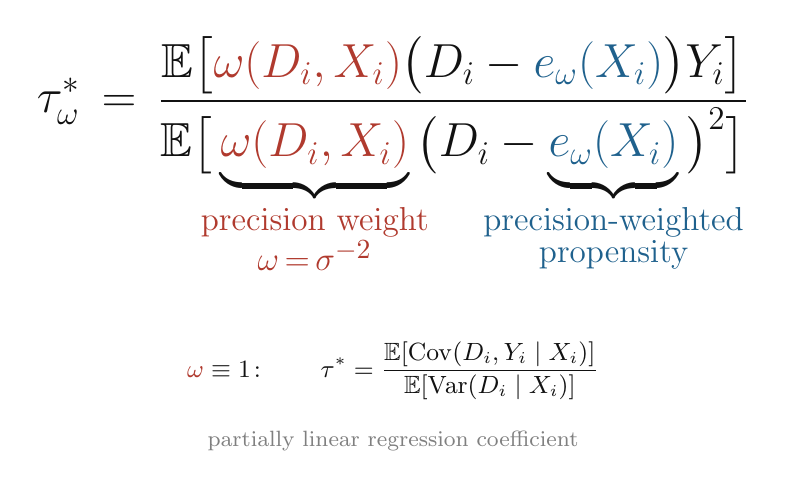
\begin{tikzpicture}
\color[HTML]{111111}
% NODE 1: Theorem 1, eq. (9) -- optimal continuous balancing estimand
\node (main) {\LARGE $\displaystyle
\tau^{*}_{\omega} \,=\, \frac{\mathbb{E}\big[\textcolor{red}{\omega(D_i,X_i)}\big(D_i - \textcolor{blue}{e_\omega(X_i)}\big)Y_i\big]}
{\mathbb{E}\big[\underbrace{\textcolor{red}{\omega(D_i,X_i)}}_{\mathclap{\textcolor{red}{\substack{\text{precision weight}\\ \omega\,=\,\sigma^{-2}}}}}\big(D_i - \underbrace{\textcolor{blue}{e_\omega(X_i)}}_{\mathclap{\textcolor{blue}{\substack{\text{precision-weighted}\\ \text{propensity}}}}}\big)^{2}\big]}
$};
% NODE 2: Theorem 1(c) -- homoskedastic special case
\node[below=6mm of main] (sub) {\small $\displaystyle \textcolor{red}{\omega}\equiv 1\colon\qquad \tau^{*} = \frac{\mathbb{E}[\operatorname{Cov}(D_i,Y_i\mid X_i)]}{\mathbb{E}[\operatorname{Var}(D_i\mid X_i)]}$};
% NODE 3: PLR equivalence (p.13), attached to the omega = 1 line only
\node[below=1.5mm of sub,gray,font=\footnotesize] {partially linear regression coefficient};
\end{tikzpicture}
\end{document}
